\documentclass[a4paper,12pt]{gress}

%\usepackage[utf8]{inputenc}
\usepackage[english]{babel}
\usepackage{hyperref}

\usepackage{amsmath,amsfonts,mathtools}
\usepackage{amsthm, amssymb, esint}
\usepackage{pgfplots}
\usepackage{graphicx}
\usepackage{hyperref}
\usepackage{float}
\usepackage{subcaption}
\usepackage{enumitem}
\usepackage{centernot}

% For displaying code
\usepackage{listings}
\usepackage{color}

\definecolor{dkgreen}{rgb}{0,0.6,0}
\definecolor{gray}{rgb}{0.5,0.5,0.5}
\definecolor{mauve}{rgb}{0.58,0,0.82}

% Settings for displaying code
\lstset{frame=tb,
  language=Python,
  aboveskip=3mm,
  belowskip=3mm,
  showstringspaces=false,
  columns=flexible,
  basicstyle={\small\ttfamily},
  numbers=none,
  numberstyle=\tiny\color{gray},
  keywordstyle=\color{blue},
  commentstyle=\color{dkgreen},
  stringstyle=\color{mauve},
  breaklines=true,
  breakatwhitespace=true,
  tabsize=3
}
\lstset{language=C++,
  basicstyle=\ttfamily,
  keywordstyle=\color{blue}\ttfamily,
  stringstyle=\color{red}\ttfamily,
  commentstyle=\color{green}\ttfamily,
  morecomment=[l][\color{magenta}]{\#}
}

% Personal definitions
\newcommand{\lra}{\ensuremath{\longrightarrow{}}}
\newcommand{\vect}[1]{\mathbf{#1}}
\renewcommand{\qedsymbol}{\rule{0.7em}{0.7em}}
\newcommand{\tabitem}{~~\llap{\textbullet}~~}
\newcommand\ddfrac[2]{\frac{\displaystyle #1}{\displaystyle #2}}

% Theorem commands
\newtheorem{lem}{Lemma}
\newtheorem{thm}{Theorem}
\newtheorem{defn}{Definition}


\title{MakeUofT 2020 Reflection}
\author{Sean Wu}
\date{February 2020}
\version{1.0}
\begin{document}

\begin{titlepage}

\maketitle

\begin{goals}{Hackathon Goals}
\begin{enumerate}
  \item Meet new people ✅
  \item Complete a Minimum Viable Product ✅
  \item Learn new hardware skills ❌
  \item Learn MongoDB ✅
  \item Deploy something on Google Cloud ✅
\end{enumerate}
\end{goals}

\newpage

\tableofcontents

\end{titlepage}

\week{Week 1 (Feb 10-16)}

\subsection{Sat-Sun Feb 15 (MakeUofT)}
First day of MakeUofT. Caught up a lot on sleep before so we'll see how this goes... We started off a little stuck as we had to choose what to work on, but we eventually decided to work on an Internet of Things project mixed in with some basic Computer Vision and full stack web design. This was a very interesting project as it had many parts and integration of all those parts was definitely the hardest part.

The basic premise of the project was to improve the studying experience of students in Myhal by dealing with issues of motion-activated lights turning off when studying and the difficulty of finding seats during peak hours. We ended up focusing more on the lights issue, which may have hurt us during presentations because we kinda lost the "wow" factor.

The first thing that I worked on was getting a basic computer vision software working in Python so that we could recognize people and count the number of people in an image. I initially had some issues with this other script that made my whole Python software go crazy for some reason. I'll definitely need to learn how to use Python virtual environments sometime soon to prevent a similar issue in the future.

I then later tried another method using a pretrained \lstinline{PeopleDetector} from work done in \lstinline{OpenCV}'s \lstinline{HOGDescriptor}. Most of it was actually just some straightforward code to draw the initial bounding box and count the number of bounding boxes drawn with just one or two lines to actually use the computer vision model.

An interesting method from the tutorial I used was using \lstinline{non_max_suppression} from the related python package \lstinline{imutils} to combine overlapping bounding boxes. This was a useful improvement as sometimes multiple bounding boxes would be drawn for each person and this function prevented any double counting.

I got this whole computer vision running pretty quickly in about an hour after the initial mess. Furthemore, I was able to spend 10-15 mins playing with different parameters to identify the best ratio of accuracy (false positives and false negatives to computing time (or at least something close enough). I ended up biasing towards having more false negatives than false positives (i.e. identify random stuff as people) because I wanted a more sensitive system. Some of my rationale for that bias was also that if the system recognized some stuff, it was probably somebody's belongings and that would mean that was someone there. Even so, there were a lot of missed cases, so in the future it would be better to train a custom model on a larger dataset with more people in different positions (standing, sitting, back turned towards camera, partially obscured, etc).

Here is some of the example output that the computer vision software got on some test images of Myhal that I pulled from Google Images.

\begin{figure}[H]
  \begin{center}
  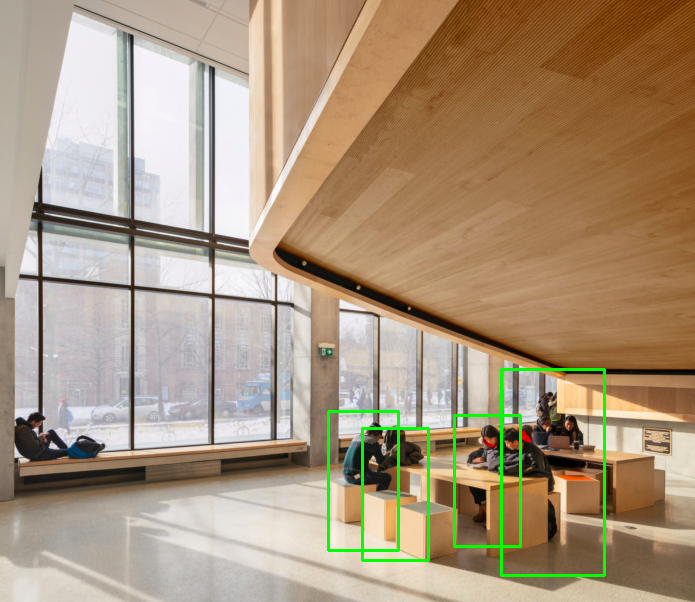
\includegraphics[width=100mm, scale=0.2]{pictures/myhal1.png}
  \caption{Example output of the basic computer vision software. Notice how it does pretty well on the people sitting at the tables even though part of their body is obscured, but it fails completely on the guy sitting near the window. Probably the dataset for the pretrained model didn't have any example of people sitting in that position but had some examples of people sitting at the table.}
  \end{center}
\end{figure}

\begin{figure}[H]
  \begin{center}
  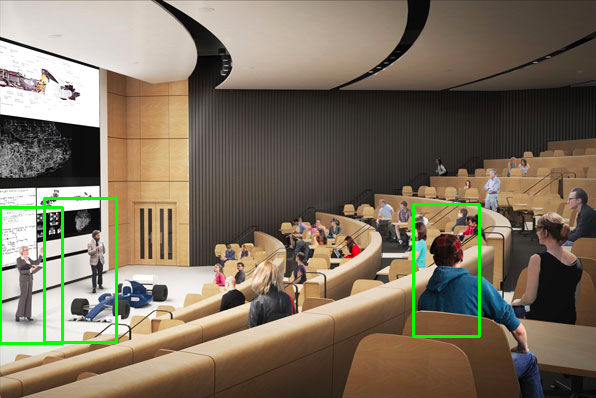
\includegraphics[width=100mm, scale=0.2]{pictures/myhal2.png}
  \caption{Example output of the basic computer vision software. This time the pretrained model does terribly. It seems to require fully body pictures of people to recognize them. Given that most of these people only have their heads showing in the image, I guess it makes sense why it's doing so bad.}
  \end{center}
\end{figure}

\begin{figure}[H]
  \begin{center}
  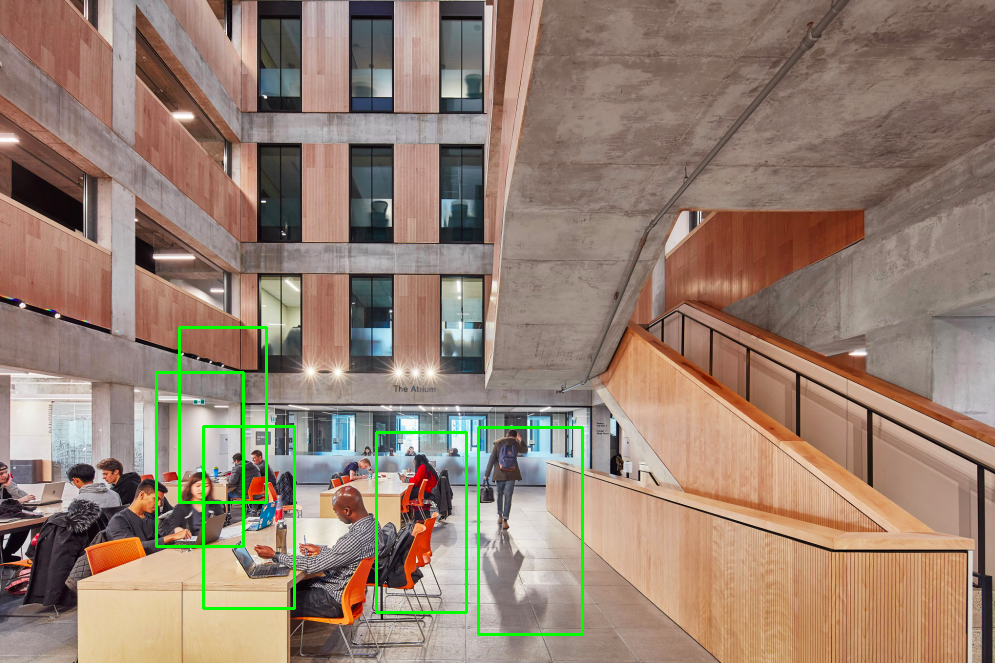
\includegraphics[width=100mm, scale=0.2]{pictures/myhal3.png}
  \caption{Example output of the basic computer vision software. Here the software does pretty decently. The bounding boxes are kinda weirdly place but there's no false positives. It did pretty poorly on the left there, but there's enough people recognized to at least get a good chunk of them.}
  \end{center}
\end{figure}

\begin{figure}[H]
  \begin{center}
  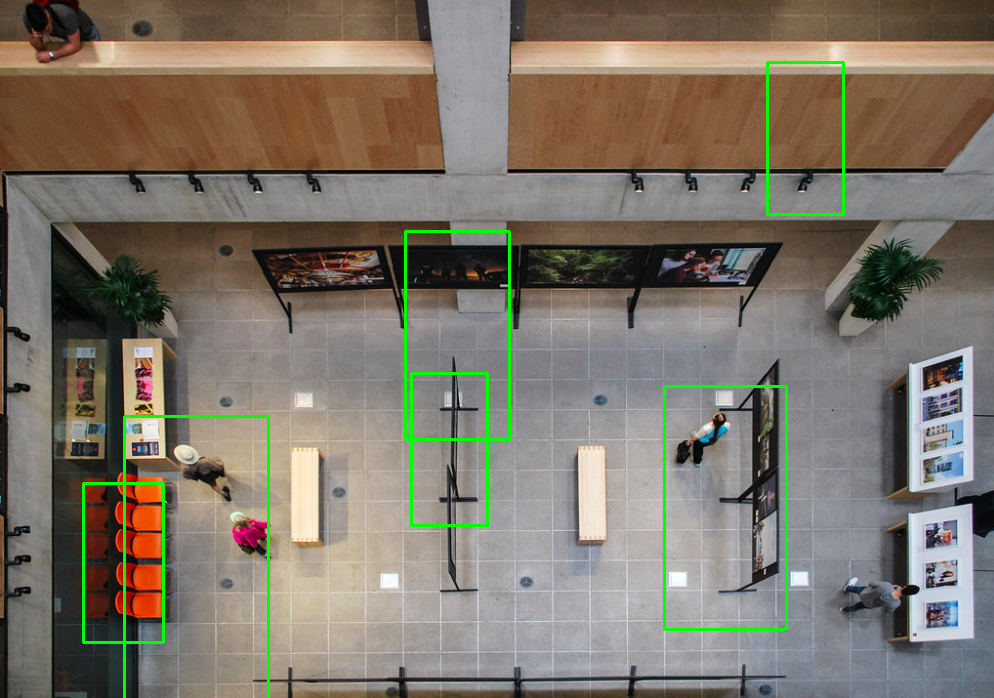
\includegraphics[width=100mm, scale=0.2]{pictures/myhal4.png}
  \caption{Example output of the basic computer vision software. Here you can see the effects of the bias towards more false positives than negatives. There are definitely a lot of objects being identified as people. Interestingly, I actually used this specific picture as one of the test images to see how bad the false positives were getting. It's also interesting that the software works pretty well at detecting actual people from this higher up angle. If this thing were to be actually implemented, it would probably be from this a high up angle like this, so this is good to see.}
  \end{center}
\end{figure}

After the relatively successful computer vision work, I then got started on implementing the full stack website design for the study space availability part of our idea. I initially thought this would be the easy and straightforward part but I could not be more wrong.

The first step was identifying what software technologies I wanted to use. Since we wanted to go for the MongoDB award, I ended up going with a MERN stack (MongoDB, ExpressJS, ReactJS, and NodeJS) since we needed something dynamic and this stack seemed to be pretty well known and understood in online tutorials and StackOverflow.

Most of my work on the hackathon ended up being working on this website. The tutorial I used split the web design into a front end and a backend. I started on the backend first where I spent a lot of time learning about MongoDB and their NoSQL database structure. While I didn't think much about the split front/server design in the beginning, it seems like a pretty good way to do separation of concerns and to modularize the design.

Since my website would only need to pull data from our \lstinline{MongoDB} database, my backend only had read access and purely used \lstinline{GET} requests to work. The database design that my teammate Jun Ho suggested was to make \lstinline{Workspaces} the overarching database, buildings like \lstinline{Myhal_Centre} and \lstinline{Bahen} the collections, and each area like the \lstinline{7th} floor to be the documents. This design ended up working very well as each building was just another collection and then I could make different queries to find specific info about all or some of the floors in each building. In the end though, I really only needed to get all the workspaces in each building. The hard part here was mostly determining how to access the documents and then figuring out the routing with \lstinline{Express} to get the server to send JSON data for each api request.

\begin{figure}[H]
  \begin{center}
  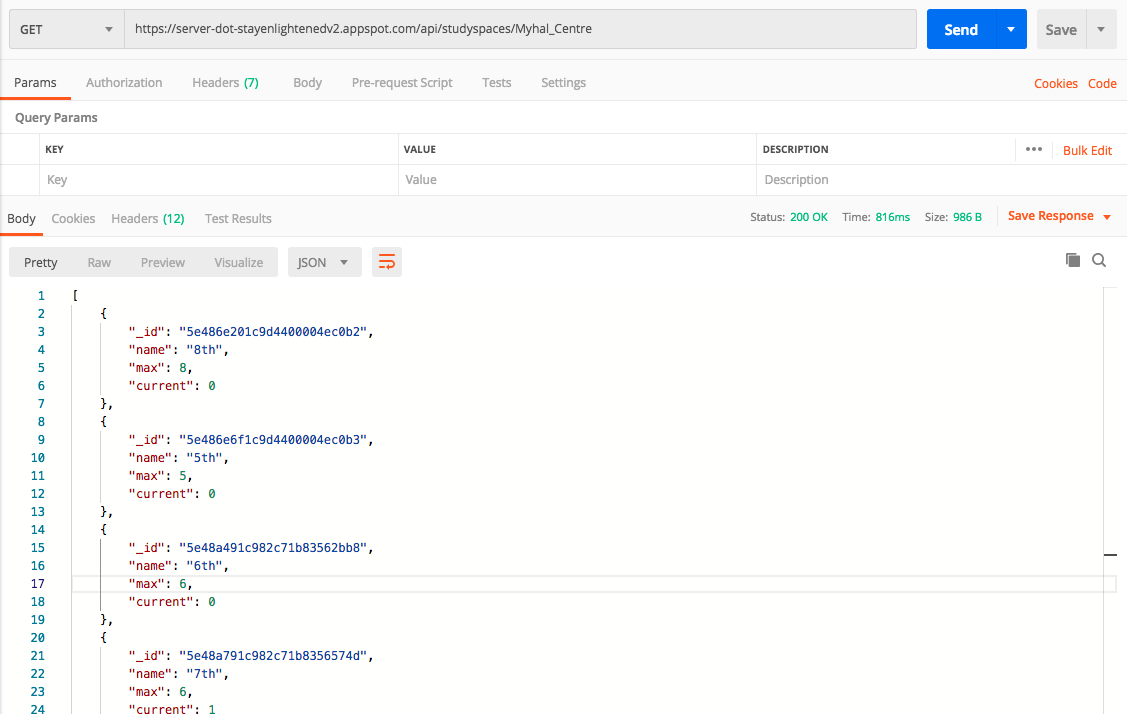
\includegraphics[width=150mm, scale=0.2]{pictures/server-api-call.png}
  \caption{Example output of making an api call to server backend of the final product. Here an api GET request for all the studyspaces in Myhal is being made and the server returns data from the MongoDB database as JSON.}
  \end{center}
\end{figure}

I lost track of time how long the rest of this took, but I definitely spent a few hours on the backend alone. But once this was working, it was time to switch to getting a working front end going. I probably spent about a similar amount of time on the front end, but it was less interesting. Here my client made api calls to my backend to get the JSON data that it could then display appropriately. The part that definitely took the longest here was displaying the JSON data for all the workspaces in Myhal. The original tutorial suggested a React package called react-table, but the issue was that the newest version did things differently and I didn't have the time to figure it out. So I was fortunately able to find an older version to run and eventually got something looking like this:

\begin{figure}[H]
  \begin{center}
  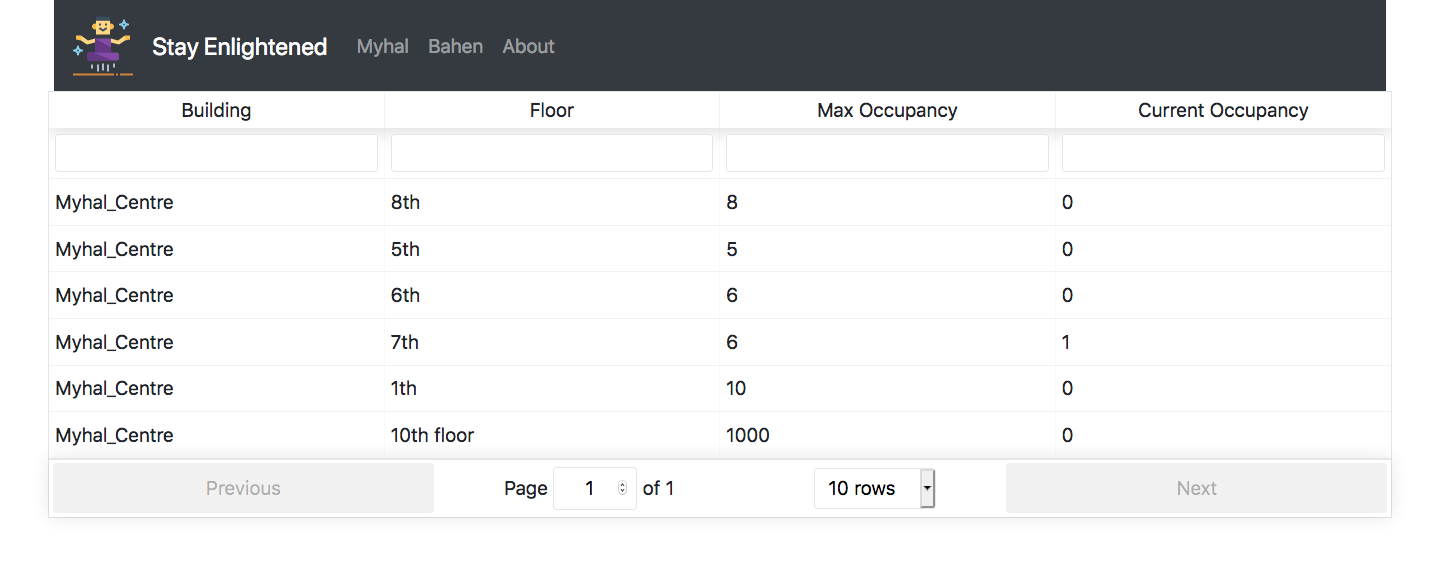
\includegraphics[width=150mm, scale=0.2]{pictures/client.png}
  \caption{Example page of front end design. Basically I just needed this table to work and then this react-table package did all the rest with making a sleek interactive table.}
  \end{center}
\end{figure}

Once I got this table working, I switched over to the actual website implementation on the cloud. We once again went with another technology with a sponsor prize as we decided to use Google Cloud. We also got a \$50 coupon for Google Cloud, so that made our decision pretty easy. To make things simple, I used Google Cloud's App Engine NodeJS environment. While I expected this to be very straightforward, I probably spent the most time here (notice a pattern lol). This was definitely very frustrating as I was already running on low sleep and I wasn't able to find the appropriate Google Cloud guides until very late (I need to get better at searching things up). During this painful process, I got a good amount of exposure to Google's cloud shell which was actually pretty nice to use.

I struggled a lot with this part because my design required both the front end and back end server to be up and running concurrently. I could get them working individually, but it would all fall apart when I put them together. The solution in the end was actually pretty short and nice; I just needed to run each one as another service for the main app.


\begin{figure}[H]
  \begin{center}
  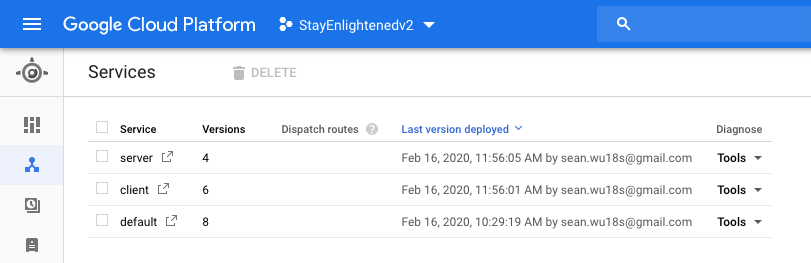
\includegraphics[width=150mm, scale=0.2]{pictures/gcp-app.png}
  \caption{Screenshot of the 3 services being run on Google's App Engine. Notice that this is actually the 2nd version of the web app because the first one failed to work properly. Also note how close the final versions were to the 12 PM lunchtime deadline.}
  \end{center}
\end{figure}


Anyways, setting this up web app on Google Cloud ending up taking most of the time and while I had tried getting it to work with a custom domain (another sponsor prize and hackathon promotion deal), that ended up not working. So I spent my time working on the front end, but by that time I was far from effective (lack of sleep and time crunch) so the end result was pretty meh.

\begin{figure}[H]
  \begin{center}
  
\includegraphics[width=150mm, scale=0.2]{pictures/final-website.png}
  \caption{Screenshot of final website design before I ran out of time. All I really changed was adding the links at the top and putting this weird picture on the homepage.}
  \end{center}
\end{figure}

This ended up being the final product of the 24 hours of work that I put in. The lack of aesthetic appeal definitely hurt our presentation but I'm still proud that it ended up being pretty functional in the end.

Presentations were also pretty mixed. There were a few that I thought pretty well, but I think we failed to fully capture their attention. I guess hackathons aren't 100\% about the tech and they definitely require strong presentation skils.

While we didn't win anything, it was still a very good experience and I got to meet some cool new people and learn more about full stack web development. It's kinda weird that I spent 24 hours (20 hours of front end) on software programming at a hardware design hackathon, but I still learnt a ton. Now that I have a full web app working, implementing something in the future should be much much more efficient and streamlined. I'm also quite interested to see what the actual cost of running this web app over a few weeks will be as it might be an option that I consider in the future. When I do check on it, I should definitely remember to shut it off so that I don't need to keep paying it.


\begin{gress}
  \moonshot{Learn Python virtual environments}
  \todo{Check costs of Google Cloud.}
  \spicy{Deployed a full web app on Google Cloud}
  \win{Finished another hackathon and met cool new people to learn from}
  \issue{Pulled an all nighter with only a 30 min nap in the afternoon. About 36 hrs without sleep}
\end{gress}

\end{document}
